% !TeX root = 00General.tex

\documentclass
[
a4paper,
openright,                    % Kap.beginn immer rechts! (fkt. nur bei report, nicht bei article)
12pt                          % ersatzweise 12pt, wenn mehr Seiten entstehen sollen
]
{report}

%%%%%%%%%%%%%%%%%%%%%%%%%%%%%%%%%%%%%%%%%%%%%%%%%%%%%%%%%%%%%%%%%%%%%%%%%%%%%%%%%%%%%%%%%%%%%%%%%%%%%%%%%%%%
%Dokumenteneigenschaften

\newcommand{\Author}{} 
\newcommand{\Title}{}
\newcommand{\Keywords}{}

%%%%%%%%%%%%%%%%%%%%%%%%%%%%%%%%%%%%%%%%%%%%%%%%%%%%%%%%%%%%%%%%%%%%%%%%%%%%%%%%%%%%%%%%%%%%%%%%%%%%%%%%%%%%
% Layout zusammengestellt von Richard Wanger im WS 2015/2016. Verschiedene Vorlagen wurden bei der Erstellung
% kombiniert und nach dem Masterleitfaden (Stand: Oktober 2015) adaptiert. Verwendung ohne Gewähr!

\usepackage{style}		%alle packages und Formatvorlagen befinden sich in dieser Datei


%%%%%%%%%%%%%%%%%%%%%%%%%%%%%%%%%%%%%%%%%%%%%%%%%%%%%%%%%%%%%%%%%%%%%%%%%%%%%%%%%%%%%%%%%%%%%%%%%%%%%%%%%	%%%
% ORGANISATORISCHES

\begin{document}
\begin{titlepage}

\hspace{7cm}

\begin{figure}[!ht]
	\centering
	
\includegraphics[width=0.3\textwidth]{fhs_logo_web.png}
\end{figure}

\begin{center}
	\vspace{2cm}
	\Huge Laboratory II
	
	\Large{\bf\large Binna, Reschenhofer, Schörghofer}
	\vspace{1cm}

	\large Course: Internet Infrastructure and Security 
	
	\large Lecturer: FH-Prof. DI Mag. Dr. Dominik Engel 
	
	\large 23.11.2016
\end{center}

%\vfill
\end{titlepage}

%%%%%%%%%%%%%%%%%%%%%%%%%%%%%%%%%%%%%%%%%%%%%%%%%%%%%%%%%%%%%%%%%%%%%%%%%%%%%%%%%%%%%%%%%%%%%%%%%%%%%%%%%%%%
%VERZEICHNISSE

\pagenumbering{roman}
\thispagestyle{plain}
\pagestyle{plain}

\tableofcontents
%\protect \addcontentsline{toc}{chapter}{Table of Contents}

%\renewcommand{\nomname}{List of Abbreviations}
%% !TeX root = 00General.tex

\chapter*{List of Abbreviations}
\addcontentsline{toc}{chapter}{List of Abbreviations} 
\pagestyle{plain}

\begin{acronym}[VLAN123]
 \acro{ARP}{Address Resolution Protocol}
 \acro{CD}{Collision Detection}
 \acro{CRC}{Cyclic Redundancy Check}
 \acro{FCS}{Frame Check Sequence}
 \acro{IEEE}{Institute of Electrical and Electronics Engineers}
 \acro{MAC}{Media Access Control}
 \acro{NIC}{Network Interface Card}
 \acro{NTP}{Network Time Protocol}
 \acro{PTP}{Precision Time Protocol}
 \acro{QoS}{Quality of Service}
 \acro{RIP}{Routing Information Protocol}
 \acro{RSTP}{Rapid Spanning Tree Protocol}
 \acro{SAT}{Source Address Table}
 \acro{STP}{Spanning Tree Protocol}
 \acro{USB}{Universal Serial Bus}
 \acro{VLAN}{Virtual Local Area Network}
 \acro{MOTD}{Message of the Day}
 \acro{PVST}{Per-VLAN Spanning Tree}
 \acro{VTP}{VLAN Trunking Protocol}
 \acro{SSH}{Secure Shell}
 \acro{DHCP}{Dynamic Host Configuration Protocol}
 \acro{DCE}{Data Communication Endpoint}
 \acro{OSPF}{Open Shortest Path First}
 \acro{IP}{Internet Protocol}
 \acro{LSR}{Link State Routing}
 \acro{AS}{Autonomous System}
 \acro{TTL}{Time To Live}
 \acro{POP3}{Post Office Protocol Version 3}
 \acro{SMTP}{Simple Mail Transfer Protocol}
 \acro{SSL}{Secure Socket Layer}
 \acro{TLS}{Transport Layer Security}
 \acro{HTTPS}{Hyper Text Transport Protocol Secure}
\end{acronym}


%\listoffigures
%\protect \addcontentsline{toc}{chapter}{List of Figures}

%\listoftables
%\protect \addcontentsline{toc}{chapter}{List of Tables}

%\lstlistoflistings
%\protect \addcontentsline{toc}{chapter}{Listingverzeichnis}

%%%%%%%%%%%%%%%%%%%%%%%%%%%%%%%%%%%%%%%%%%%%%%%%%%%%%%%%%%%%%%%%%%%%%%%%%%%%%%%%%%%%%%%%%%%%%%%%%%%%%%%%%%%%
%INHALT

%\clearpage
%\pagenumbering{arabic}
%\chapter{Beispiele}

\thispagestyle{standard}
\pagestyle{standard}

\section{Text und Zitate}

In Moby-Dick geht es in erster Linie um die Jagd auf einen weißen Pottwal \footnote{nach: https://de.wikipedia.org/wiki/Moby-Dick}. Kurze Zitate (unter drei Zeilen) müssen mit Anführungszeichen gekennzeichnet werden. Außerdem müssen die Quelle sowie die Seite angegeben werden. Ein Beispiel für ein kurzes Zitat: \glqq Komisch. Manch einer von uns wünschte sich, er lebe auf einer Südseeinsel.\grqq \cite{MELVILLE:MOBYDICK1997} (Seite 100).

  \begin{quote}
"Das Buch hier Lieblingsbuch. Viele Blätter viele, schöne Bilder. Du kennen Worte?"\newline
"Ja"\newline
"Ich kennen Bilder. Das ein Wal. Du lesen Worte!"\newline
"Durch das Herz des Wals strömt mehr Flüssigkeit als durch das große Wasserleitungsrohr unter der London Bridge, jedoch strömt das Wasser nicht so stark, wie das Blut, das vom Herz des Wals pocht."\newline
"Du gut, ich danken dir."  \upshape \cite{MELVILLE:MOBYDICK1997} (Seite 500)
  \end{quote}

Ein sehr praktisches Package ist cleveref. Es automatisiert und erleichtert das setzen von Referenzen ungemein. Als Beispiel wird eine Referenz auf das FHS-Logo gesetzt siehe \cref{FIG_LOGO}.

Für das Verfassen von wissenschaftlichen Arbeiten können eine Vielzahl an Quellentypen herangezogen werden. Beispiele hierfür sind Leitfäden (Manuals) \citep{RFC2828} \citep{80211i} \citep{80211} \cite{X800} \citep{TR102377} \citep{EN301893} \citep{PUB197} \citep{PUB74}, Bücher \citep{Fis04a} \citep{Rei05a} \citep{Tan00a} \citep{Ste04a} \citep{GMS00a} \citep{HL98a}, Sammelbände \citep{EHL00a} \citep{Sch94a}, Journal-Artikel \citep{TM03a} \citep{CP03a}, Konferenz-Proceedings \citep{HCB00a} \citep{KBW04a} \citep{KSW04a} \citep{HK05a}, Internetmagazine \citep{Eke05a}, Webquellen \cite{nist} \cite{php} \cite{BDKMT93a} \cite{IDSSM} sowie Diplomarbeiten und Dissertationen \citep{Sch98} \cite{Hae94a}.

Als Beispiel für eine Abkürzung wird hier \ac{ADF} angeführt. Das Package schreibt automatisch das erste Vorkommen der Abkürzung aus. Die zweite Verwendung von \ac{ADF} wird also abgekürzt. Ist ein Ausschreiben einer Abkürzung gewünscht wird der acl-Befehl verwendet. Dies führt zu \acl{ADF}. Abkürzungen müssen in der Datei \glqq 05Abkuerzungsverzeichnis\grqq angegeben werden.

\section{Quelltext}

\texttt{printf("Hallo Welt")} für Ausschnitte von Sourcecode innerhalb von Text

\lstset{escapeinside={\%*}{*)},numbers=none}%oder numbers=left
\begin{lstlisting}[language=C,
caption=Beispiel-Listing,
label=LST_SAMPLE]
serverTCP = new TcpListener(IPAddress.Parse(serverIP), serverPort);
\end{lstlisting}

\lstset{escapeinside={\%*}{*)},numbers=left}
\lstinputlisting[language=Matlab, caption=Einfaches Matlabprogramm in einer Datei, label=list:hello.m]{Listings/hello.m}

\section{Bilder}

\begin{figure}[H]
\begin{center}
	
\includegraphics[scale=0.4]{BilderAllgemein/Logo.jpg}
\end{center}
	%\includegraphics[width=\textwidth]
	%\end{center}
	% Title
	\caption{Das FHS-Logo}
	% Unique name: identifier for referencing
	\label{FIG_LOGO}
\end{figure}

\section{Formeln}

Formeln sind für jeden Abschnitt rechtsbündig von dieser zu nummerieren, um einen späteren Bezug in der Arbeit zu gewährleisten. Formeln werden üblicherweise in "`Computer Modern Roman"' (\LaTeX{}-Standard) gesetzt. In diesem Template wird die Formel-Schrift bzw. das Package \texttt{eulervm} verwendet. Abgesetzte Formeln werden in \LaTeX{} durch die 
\emph{equation} Umgebung definiert. Formelausdrücke innerhalb von Textabschnitten erhält man durch \$Formel\$.

\subsection*{Beispiel}
%
Der \emph{Sinus cardinalis} oder sinc-Funktion ist eine mathematische Funktion $f$, welche in nicht-normierter Version als

\begin{equation}
	f(x) := \frac{\sin(x)}{x}
	\label{eq:bsp}
\end{equation}

definiert wird. In der digitalen Signalverarbeitung findet meistens nachfolgende normierte Version $\mathrm{si}(x)$ oder $\mathrm{sinc}(x)$ Anwendung \cite{x1}, \cite{x2}. Für eine Visualisierung dieser Funktionen siehe Abb.~\ref{FIG_LOGO}.

\begin{equation}
	f(x) := \frac{\sin(\pi x)}{\pi x}
	\label{EQ_SAMPLE}
\end{equation}

\section{Beispiel für Tabellen}
%
Es empfiehlt sich, für Tabellen die Standard-\LaTeX{}-Umgebung \emph{tabular} zu verwenden. Bei Bedarf können natürlich auch Erweiterungen (z.B.~\emph{tabularx} oder \emph{array}) zur Anwendung kommen. Eine mögliche Darstellung zeigt Tabelle \ref{Table_Sinc}.

\begin{table}[h!]%
	\begin{center}
		\begin{tabular}{|r|r|r|}
			\firsthline
			$x$&$\mathrm{sinc}(x)$&$\mathrm{sin}(x)$\\\hline\hline
			$-0.5$&0.6366&-0.4794\\\hline
			$0$&1.0000&0\\\hline
			$0.5$&0.6366&0.4794\\\hline
		\end{tabular}
		\caption{Zwei Werte der Sinc-Funktion}
		\label{Table_Sinc}
	\end{center}
\end{table}










\clearpage
\pagenumbering{arabic}

\renewcommand{\nomname}{Abkürzungsverzeichnis}
% !TeX root = 00General.tex

\chapter*{List of Abbreviations}
\addcontentsline{toc}{chapter}{List of Abbreviations} 
\pagestyle{plain}

\begin{acronym}[VLAN123]
 \acro{ARP}{Address Resolution Protocol}
 \acro{CD}{Collision Detection}
 \acro{CRC}{Cyclic Redundancy Check}
 \acro{FCS}{Frame Check Sequence}
 \acro{IEEE}{Institute of Electrical and Electronics Engineers}
 \acro{MAC}{Media Access Control}
 \acro{NIC}{Network Interface Card}
 \acro{NTP}{Network Time Protocol}
 \acro{PTP}{Precision Time Protocol}
 \acro{QoS}{Quality of Service}
 \acro{RIP}{Routing Information Protocol}
 \acro{RSTP}{Rapid Spanning Tree Protocol}
 \acro{SAT}{Source Address Table}
 \acro{STP}{Spanning Tree Protocol}
 \acro{USB}{Universal Serial Bus}
 \acro{VLAN}{Virtual Local Area Network}
 \acro{MOTD}{Message of the Day}
 \acro{PVST}{Per-VLAN Spanning Tree}
 \acro{VTP}{VLAN Trunking Protocol}
 \acro{SSH}{Secure Shell}
 \acro{DHCP}{Dynamic Host Configuration Protocol}
 \acro{DCE}{Data Communication Endpoint}
 \acro{OSPF}{Open Shortest Path First}
 \acro{IP}{Internet Protocol}
 \acro{LSR}{Link State Routing}
 \acro{AS}{Autonomous System}
 \acro{TTL}{Time To Live}
 \acro{POP3}{Post Office Protocol Version 3}
 \acro{SMTP}{Simple Mail Transfer Protocol}
 \acro{SSL}{Secure Socket Layer}
 \acro{TLS}{Transport Layer Security}
 \acro{HTTPS}{Hyper Text Transport Protocol Secure}
\end{acronym}


\chapter{Topology}

\thispagestyle{standard}
\pagestyle{standard}

The following topology (figure \ref{img:topo}, taken from the Moodle instructions) had to be recreated in the lab.

\begin{figure}[H]
	\centering
	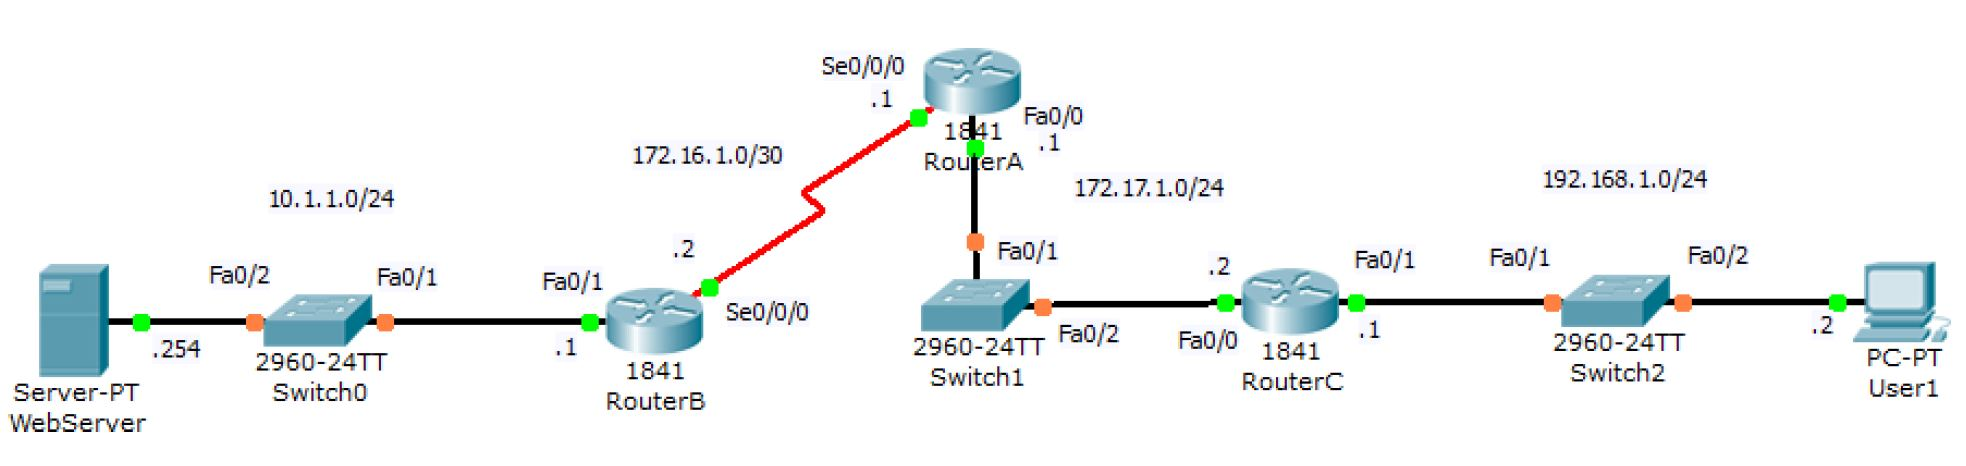
\includegraphics[width=0.9\textwidth]{img/topo.png}
	\caption{Topology (Moodle)}
	\label{img:topo}
\end{figure}

Each device was configured with basic settings like hostname, \ac{MOTD}, a secret enable password, disabled IP domain lookup, synchronous logging on line console 0 and the service password-encryption, which prevents passwords from being displayed in clear-text in the start-up and running configuration. The important part is that the clock-rate for the serial interface has to be configured on the \ac{DCE} device.

\lstset{escapeinside={\%*}{*)},numbers=left}%oder numbers=left
\begin{lstlisting}[caption={Setting the clock-rate on Router A},label={lst:clockrate},language={}]
interface Serial0/0/0
 bandwidth 64
 ip address 172.16.1.1 255.255.255.252
 ip ospf authentication message-digest
 ip ospf message-digest-key 1 md5 7 094F471A1A0A
 clock rate 64000
\end{lstlisting}

\ac{OSPF} is a routing protocol for \ac{IP} networks. It uses a \ac{LSR} algorithm and falls into the group of interior routing protocols, operating within a single \ac{AS}.
Concerning the \ac{OSPF} routing, every router assigns its known networks to the \ac{OSPF} routing process with area 0.
\newpage
\lstset{escapeinside={\%*}{*)},numbers=left}%oder numbers=left
\begin{lstlisting}[caption={\ac{OSPF} routing example router A},label={lst:ospf},language={}]
router ospf 1
 area 0 authentication message-digest
 network 172.16.1.0 0.0.0.3 area 0
 network 172.17.1.0 0.0.0.255 area 0
\end{lstlisting}

"nginx" has been set up as a webserver on a linux pc with default configuration for http (IP address for the webserver is "10.1.1.254"). Ping and webserver access from the user-pc to the webserver has been successful as shown in (figure \ref{img:GuterWebserverScreenshot}). Be sure to disavle the windows firewall on both devices to allow ping.

\begin{figure}[H]
	\centering
	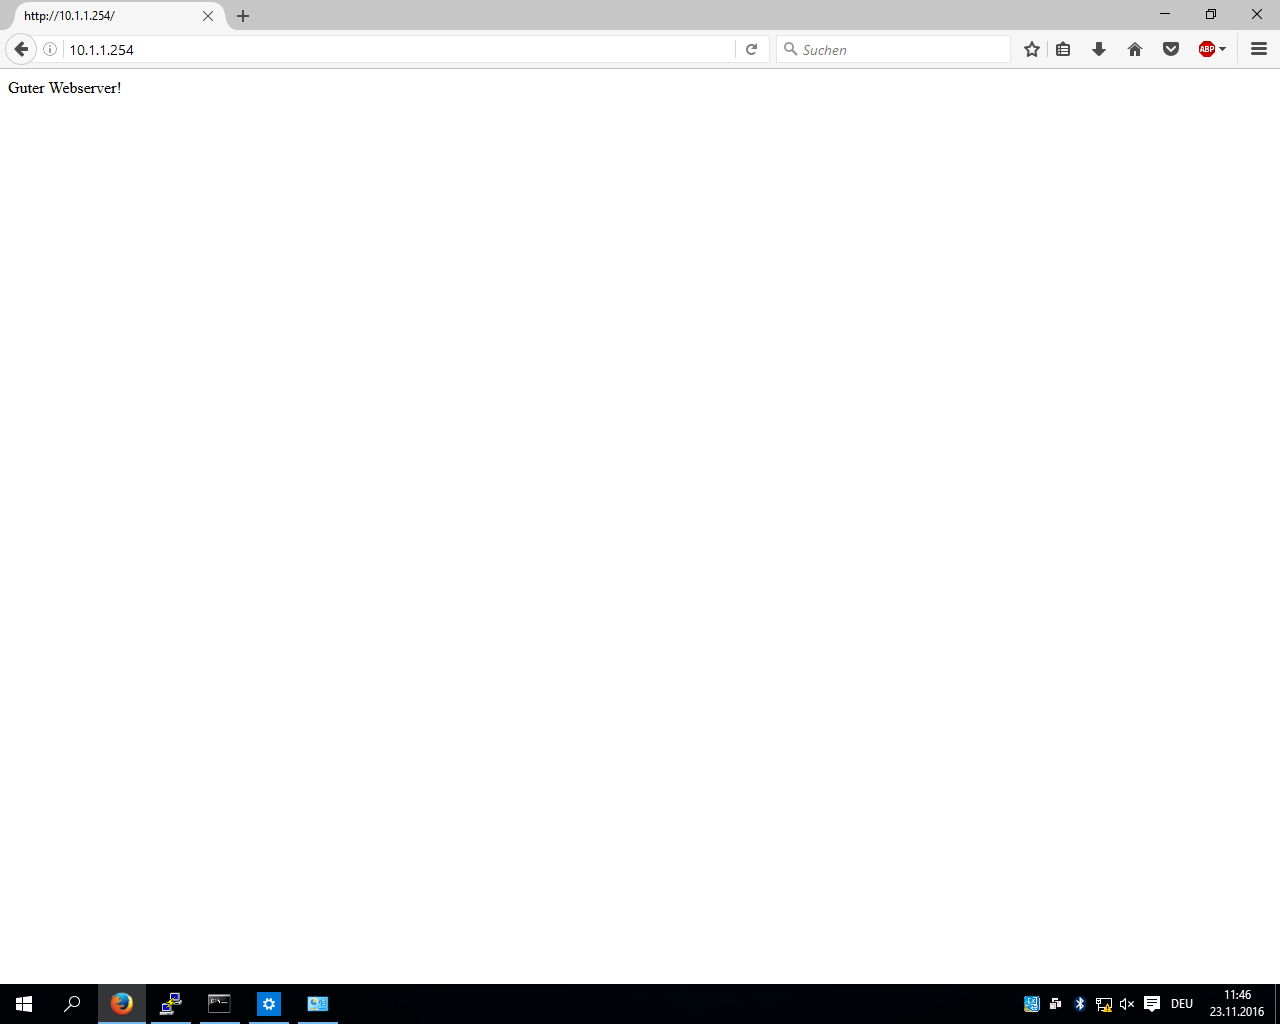
\includegraphics[width=0.9\textwidth]{img/GuterWebserverScreenshot.png}
	\caption{Webserver access}
	\label{img:GuterWebserverScreenshot}
\end{figure}

For this topology the ping command from the user pc to the webserver took on average 18ms and had a remaining \ac{TTL} of 61.
The tracert command as shown in (figure \ref{img:TracertGuterWebserver}) from the user pc to the webserver shows that a package needs 4 hops to reach the webserver.

\begin{figure}[H]
	\centering
	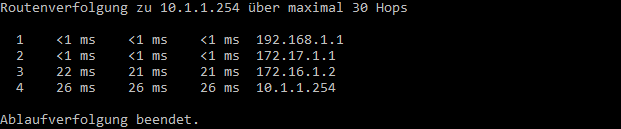
\includegraphics[width=0.9\textwidth]{img/TracertGuterWebserver.png}
	\caption{Tracert from user pc to good webserver}
	\label{img:TracertGuterWebserver}
\end{figure}

\chapter{Router Spoofing}

For the router spoofing attack another router has beed added to the network as seen in (figure \ref{img:Router spoofing topology}, taken from the Moodle instructions). This router also operates in \ac{OSPF} mode. 

\begin{figure}[H]
	\centering
	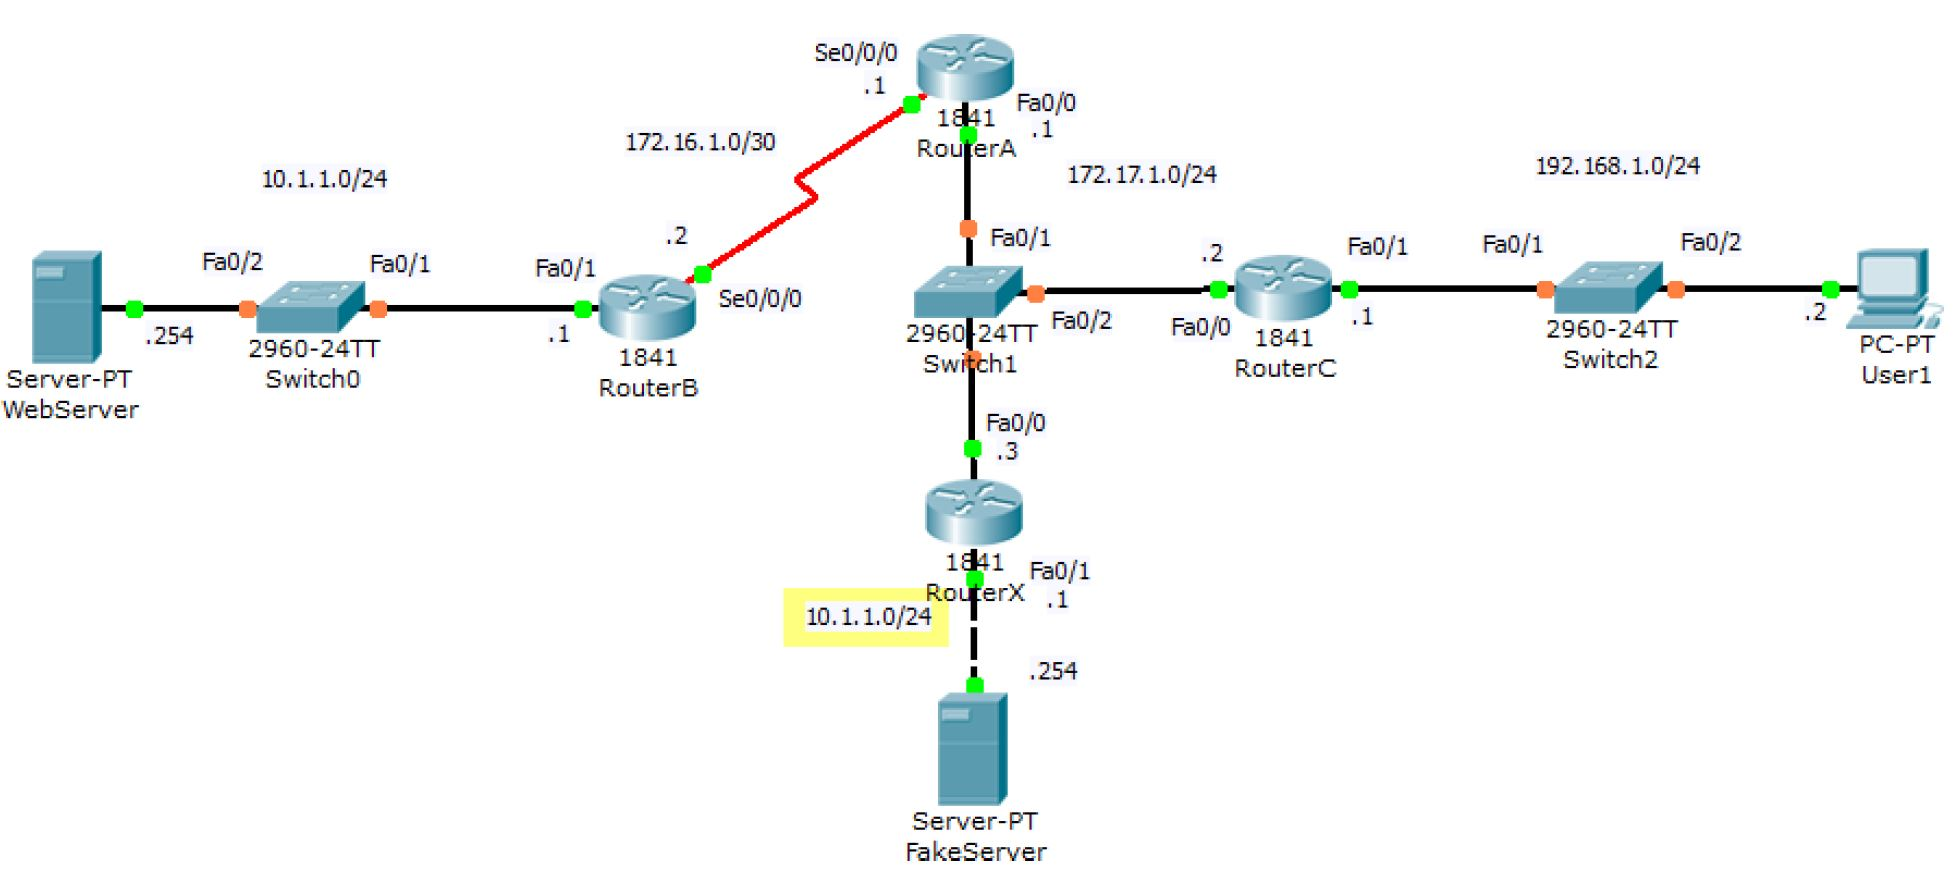
\includegraphics[width=0.9\textwidth]{img/topo_spoofing.png}
	\caption{Router spoofing topology}
	\label{img:Router spoofing topology}
\end{figure}

Router X is now configured in a way that neighboring routers think this Router B with the webserver in his network. 

\lstset{escapeinside={\%*}{*)},numbers=left}%oder numbers=left
\begin{lstlisting}[caption={\ac{OSPF} configuration on router X},label={lst:ospfRouterX},language={}]
router ospf 1
 network 10.1.1.0 0.0.0.255 area 0
 network 172.17.1.0 0.0.0.255 area 0
\end{lstlisting}

\ac{OSPF} detects changes in the topology it computes the shortest-path tree for each route using a method based "Dijkstra's algorithm". The bad Router X propagates that he has a network "10.1.1.0/24" with the webserver. This results in a shorter path from the user pc to the webserver. The user pc doesn't know that this is a bad webserver since \ac{OSPF} only detected a shorter path to the webserver. Router C is now storing the route to Router X in the routing table, because this route has the lower path cost. Therefore, a ping from the user pc now goes to the bad server.
The ping from the user pc to the bad webserver is <1ms with a TTL of 62. Because of the new route the package isn't sent over the serial link whichg results in a shorter response time for the ping command. The tracert command (figure \ref{img:TracertBadWebserver}) shows that the package only needs 3 hops to its destination and the averga response time is <1ms.

\begin{figure}[H]
	\centering
	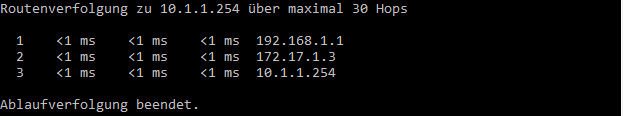
\includegraphics[width=0.9\textwidth]{img/TracertBadWebserver.png}
	\caption{Tracert from user pc to bad webserver}
	\label{img:TracertBadWebserver}
\end{figure}

If the user wants to access the webserver again, he will be redirected to the bad webserver, because of the routing table entry in router C which states that the shortest path to the network "10.1.1.0/24" with the webserver is the one via router X.
(figure \ref{img:BadWebserverScreenshot}) shows the output when accessing the webserver.

\begin{figure}[H]
	\centering
	
\includegraphics[width=0.9\textwidth]{img/BadWebserverScreenshot.png}
	\caption{Bad webserver access}
	\label{img:BadWebserverScreenshot}
\end{figure}

\chapter{Router Authentication}

In this chapter, the router authentication methods are explaned. Router authentication for \ac{OSPF} allows to flexibly authenticate \ac{OSPF} neighbours. This enables \ac{OSPF} routing to exchange routing update information in a secure manner.
There exist three different types of authentication in OSPF:
\begin{itemize}
\item Null authentication: Also called type 0 -> no authentication information is included in the packet header. This is also default.
\item Plain text authentication: type 1 -> use of simple plain-text passwords
\item Md5 authentication: typ2 -> use of md5 cryptographic passwords (also not secure anymore!)
\end{itemize}

OSPFv3 is capable of using SHA1 authentication, which is at least better than MD5 authentication.

\section{Plain Text Authentication}

At first, plain text authentication has been configured.
The authentication key is configured for each interface separately by use of the following command:

\texttt{ip ospf authentication-key cisco}

Only interfaces, where the authentication key match, can participate in OSPF advertising.
The following command then enables OSPF authentication for all interfaces inside area 0:

\begin{tabbing}
\texttt{router} \= \texttt{ospf 1} \\
\> \texttt{area 0 authentication}
\end{tabbing}

When the commands above are executed on only Router A and Router C, all OSPF routes that have previously been stated in the routing table (advertised from Router B) are now lost, because Router B doesn’t have the authentication configuration.
The big disadvantage of plain text authentication is, that the password can be clearly seen in the packet.

\pagebreak
\section{MD5 Authentication}

First the md5 message digest has to be set on the interfaces:
\begin{tabbing}
\texttt{Interf}\= \texttt{ace s0/0/0} \\
\> \texttt{ip ospf message-digest-key 1 md5 cisco}
\end{tabbing}

After that, md5 authentication can either be enabled on a per interface basis with the following command:
\begin{tabbing}
\texttt{Interf}\= \texttt{ace s0/0/0} \\
\> \texttt{ip ospf authentication message-digest}
\end{tabbing}
   
Or globally for all interfaces belonging to a specific area:
\begin{tabbing}
\texttt{router} \= \texttt{ospf 1} \\
\> \texttt{area 0 authentication message-digest}
\end{tabbing}

\chapter{Sniffing Attack and Clear Text Password Router Authentication}

%%%%%%%%%%%%%%%%%%%%%%%%%%%%%%%%%%%%%%%%%%%%%%%%%%%%%%%%%%%%%%%%%%%%%%%%%%%%%%%%%%%%%%%%%%%%%%%%%%%%%%%%%%%%
% LITERATURVERZEICHNIS

%\interlinepenalty=10000 % Literatureinträge: Absätze zusammenhalten
%\clearpage
%\addcontentsline{toc}{chapter}{Literatur}
%\singlespace
%\bibliography{12bibliografie}
%\interlinepenalty=100

%%%%%%%%%%%%%%%%%%%%%%%%%%%%%%%%%%%%%%%%%%%%%%%%%%%%%%%%%%%%%%%%%%%%%%%%%%%%%%%%%%%%%%%%%%%%%%%%%%%%%%%%%%%%
% ANHÄNGE

\begin{appendix}
%





\end{appendix}

\end{document}